\title{2022 Summer Reading Challenge: Infinite Powers}
\author{Samarth Das (Guest Writer)}

\begin{document}
The title of the book is called “Infinite Powers.” This gives an idea of a superhero story. The
story is about the mathematical superhero. Calculus is the branch of mathematics that gives you
infinite powers; most technology nowadays is based on these simplistic ideas. It also showcases
the hardwork of many people before us; the many scientists who had the guts and wits to
pioneer an idea that at the time was considered completely absurd. It is the work of these
unique people who we rely on till date for our technology. The journey from infinity to the modern
world is one that has been ignored at large and finally is exemplified in this book.

\begin{center}
   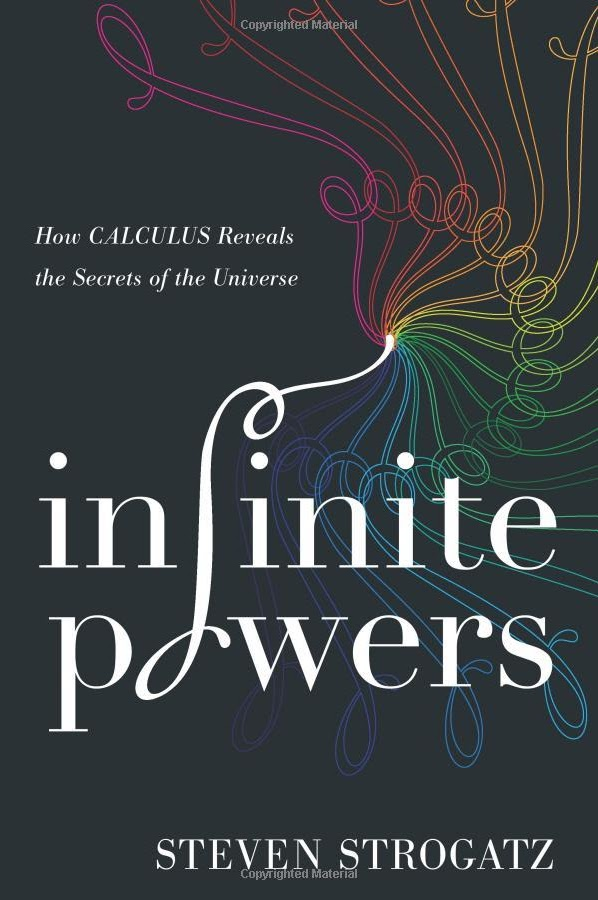
\includegraphics{images/infinity_powers.jpg}
\end{center}

The story starts off with the notion of infinity. It shows that infinity has created many issues in
ancient society, from executions to a disregarding of an entire field of mathematics. Many
ancient philosophers believed that it was something dangerous and broke all laws of
mathematics at the time. Philosophers like Zeno came up with “paradoxes” that showed how
infinity was an untamed animal. This remained for about two hundred years until Archimedes
came along. He knew how to harness infinity and work with it.
Archimedes was a pioneer of calculus because he came up with the ideas of cutting
unmeasurable objects into smaller measurable objects, an integral. He also came up with the
ideas of limits, which were essential for calculus because they proved that not all seemingly
infinite things are actually infinite. Thus concludes the ancient era of mathematics, since there
were no new developments for over eighteen hundred years.
People such as Galilieo, Descartes, and Newton came along and the mathematical
advancements rapidly developed. It started with the laws of planetary motion by Kepler. Then
Descartes arrived at the scene with the coordinate plane, a combination of algebra and
geometry. This was used by Newton to devise the laws of motion. With this came the great
acceleration of mathematics during the Scientific Revolution. Calculus was official now with
Leibiniz and Newton’s work, and it started to spill into other fields.
Calculus became quickly essential in the engineering field. Construction of automatons and
other machines such as trains were made much more efficient. It was an important part of the
First Industrial Revolution. Then came World War I and II, where the technological
advancements were heavily used. The atomic bomb would not have been possible without
calculus insight, and so would much of our military equipment today ranging from satellite
systems to tanks. Following this came the Cold War. Advancements such as in the Space Race
would not have been possible without calculus. We would have never landed on the moon. As
of today, it has extended into almost all fields of science, from medicine to space.
The idea of pure mathematics being applied to other disciplines appealed to me. I recalled an
experience I had earlier regarding mathematics. As I learned calculus, I was able to apply it to
my physics studies and beyond. I realized that there is a whole new world out here; that there
are many fields of research that have stemmed from one basic idea. A story about mathematics
history transforms oneself into an omniscient.
\end{document}